\section*{VALIDATION}\label{validation}
The accuracy of the fitted models have been estimated using two test
data sets, containing 20\% and 30\% of the data. The results from this
evaluation in seen in Tab.\ref{tab:test_validataion} and
Fig.\href{fig_test_evaluation}{(below)}. The Support Vector Regressor
seems to be the model that performs the best. However, none of the
models seem to perform very well on this dataset and the accuracy
changes very much with the test size, which means that the ranking
between the models is very unreliable. So one might as well use the
simple polynomial regression. The explicit formula from this regression
is shown in Eq.\ref{eq:model_polynomial}. It can be seen from
this expression that the $Power$ depends on the ship draught $T$ and
one of the wind components $U_{wind}$. There is however also a very
high interception term, which means that most of the $Power$ is not
explained by this model, if we assume that $Power$ is zero when the
ship is at rest in the harbour.
\begin{figure}[H]
\begin{center}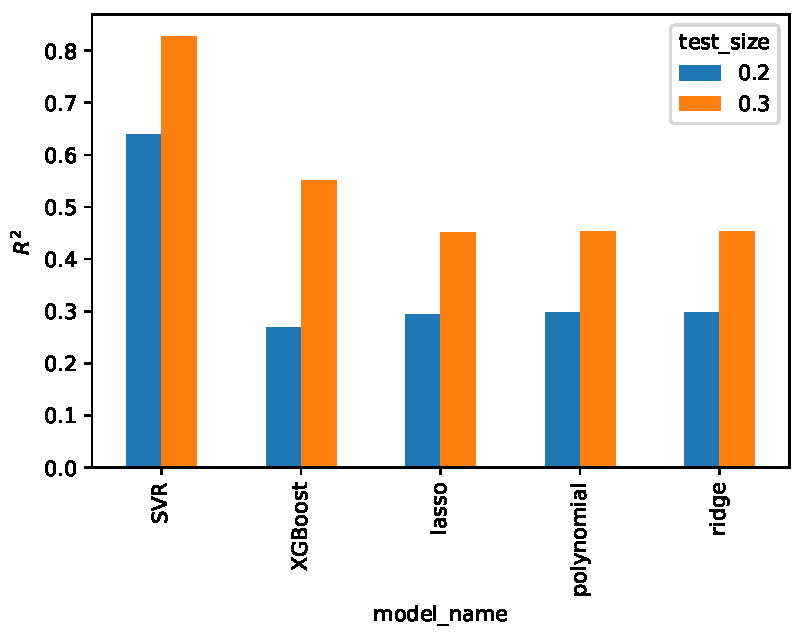
\includegraphics[width = 0.95\textwidth]{figures/test_evaluation.pdf}\end{center}
\vspace{-0.7cm}
\caption{Evaluation of the fitted models accuracy}
\label{fig:test_evaluation}
\end{figure}
\begin{figure}[H]
\begin{center}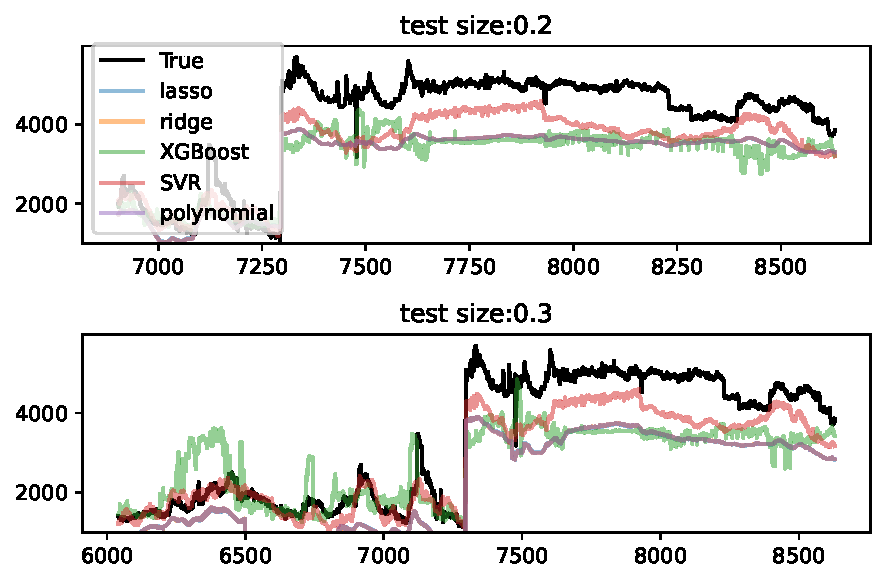
\includegraphics[width = 0.95\textwidth]{figures/output_42_0.pdf}\end{center}
\vspace{-0.7cm}
\caption{}
\label{fig:}
\end{figure}
\begin{equation}
y = - 944.923049 T + 244.319815 U_{wind} + 2964.727832
\label{eq:model_polynomial}
\end{equation}
